% Festlegung des allgemeinen Dokumentenformats
\documentclass[a4paper,12pt]{article}

% Schrift
\usepackage[T1]{fontenc}
\usepackage{lmodern}
\usepackage[utf8]{inputenc}
\usepackage[ngerman]{babel}

% Bilder
\usepackage{graphicx}
\usepackage{float}
\graphicspath{{./assets/img}}

% Variablen
% Variablen
\newcommand{\titleDocument}{Wissenschaftliche Abhandlung}
\newcommand{\subjectDocument}{Realisierbarkeit eines Upload-Filters in Bezug auf das Urheberrechts-Diensteanbieter-Gesetz am Beispiel von Grafiken}
\newcommand*{\bildquelle}{
  \footnotesize Quelle:
}
\newcommand{\code}[1]{\noindent\ignorespaces\texttt{#1}}

% Code
\usepackage{listings}
\usepackage{color}

\definecolor{black}{rgb}{0,0,0}
\definecolor{dkgreen}{rgb}{0,0.6,0}
\definecolor{gray}{rgb}{0.5,0.5,0.5}
\definecolor{mauve}{rgb}{0.58,0,0.82}

\lstset{literate=%
    {Ö}{{\"O}}1
    {Ä}{{\"A}}1
    {Ü}{{\"U}}1
    {ß}{{\ss}}1
    {ü}{{\"u}}1
    {ä}{{\"a}}1
    {ö}{{\"o}}1
    {~}{{\textasciitilde}}1
}

\lstdefinestyle{Bash} {
  frame=single,
  language=Bash,
  aboveskip=3mm,
  belowskip=3mm,
  showstringspaces=false,
  columns=flexible,
  basicstyle={\small\ttfamily},
  numbers=none,
  numberstyle=\tiny\color{black},
  keywordstyle=\color{black},
  commentstyle=\color{black},
  stringstyle=\color{black},
  breaklines=true,
  breakatwhitespace=true,
  tabsize=3
}

\lstset{emph={\$},emphstyle=\textbf}

\lstdefinestyle{Python} {
  frame=single,
  language=Bash,
  aboveskip=3mm,
  belowskip=3mm,
  showstringspaces=false,
  columns=flexible,
  basicstyle={\small\ttfamily},
  numbers=left,
  numberstyle=\tiny\color{mauve},
  keywordstyle=\color{mauve},
  commentstyle=\color{dkgreen},
  stringstyle=\color{dkgreen},
  breaklines=true,
  breakatwhitespace=true,
  tabsize=2
}

% mehrseitige Tabellen ermöglichen
\usepackage{longtable}
\usepackage{diagbox}

% Packet für Seitenrandabstände und Einstellung für Seitenränder
\usepackage{geometry}
% Internet
%\geometry{left=3.5cm, right=2.5cm, top=2.5cm, bottom=2cm}
% Kern
\geometry{a4paper, top=27mm, left=20mm, right=20mm, bottom=35mm, headsep=10mm,
footskip=12mm}

% bricht lange URLs "schön" um
\usepackage[hyphens,obeyspaces,spaces]{url}

% Festlegung Art der Zitierung
\usepackage{csquotes}
\usepackage[style=apa, backend=biber]{biblatex}
\addbibresource{./assets/literatur.bib}

% Abstand zwischen Absätze
\setlength{\parindent}{2em}
\setlength{\parskip}{1em}

% Paket für Zeilenabstand
\usepackage{setspace}
\onehalfspacing
% Kern:
% \setstretch{1.15}

% Um Itemize zu konfigurieren (kein Abstand zur Zeile davor)
\usepackage{enumitem}

% für Bildbezeichner
\usepackage{capt-of}

% für Stichwortverzeichnis
\usepackage{makeidx}

% Für Phantomsection
\usepackage{hyperref}

% Für Tabellen
\usepackage{tabularx}

% Konfiguriere das Inhaltsverzeichnis
\usepackage{tocbasic}

% Anhang: PDF einfügen
\usepackage{pdfpages}

% subsubsubsection durch paragraph
\usepackage{titlesec}
\setcounter{secnumdepth}{4}
\titleformat{\paragraph}
{\normalfont\normalsize\bfseries}{\theparagraph}{1em}{}
\titlespacing*{\paragraph}
{0pt}{3.25ex plus 1ex minus .2ex}{1.5ex plus .2ex}
% Kern:
\titlespacing{\section}{0pt}{12pt plus 4pt minus 2pt}{8pt plus 2pt minus 2pt}
\titlespacing{\subsection}{0pt}{12pt plus 4pt minus 2pt}{6pt plus 2pt minus 2pt}
\titlespacing{\subsubsection}{0pt}{12pt plus 4pt minus 2pt}{4pt plus 2pt minus 2pt}

% \autoref: Subsubsection umbenennen
\addto\extrasngerman{
    \def\subsubsectionautorefname{Unterabschnitt}
}

% Titel
\title{Wissenschaftliche Abhandlung}

% Autor
\author{Andreas Huber}

% Datum
\date{\today}

%
% Start
% des
% Dokuments
%
\begin{document}

% Titelseite
\thispagestyle{empty}

\begin{figure}[t]
 \centering
 
\includegraphics[width=0.4\textwidth]{assets/oth/logo}
\end{figure}

\begin{verbatim}
\end{verbatim}

\begin{center}
    \Large{Ostbayerische Technische Hochschule Regensburg} \\
    \Large{Fakultät für Informatik und Mathematik}
\end{center}

\begin{verbatim}
\end{verbatim}

\begin{center}
    \doublespacing
    \textbf{\huge{\titleDocument}}\\

    \onehalfspacing

    % \begin{center}
    %     Zur Erlangung des akademischen Grades \\ Bachelor of Science (B. Sc.)
    % \end{center}

    \begin{verbatim}
    \end{verbatim}

    \begin{doublespace}
        \textbf{\Large{{~\subjectDocument}}}
    \end{doublespace}
\end{center}

\vspace*{\fill}

\begin{flushleft}
    \begin{tabularx}{\linewidth}{@{}>{\bfseries}l@{\hspace{.9em}}X@{}}
        \textbf{Vorgelegt von:} & Andreas Huber <andreas.huber@st.oth-regensburg.de> \\
        \textbf{Matrikelnummer:}& 3370380 \\
        \textbf{Studiengang:}   & Master Informatik (Schwp. Software Engineering) \\
                                & \\
        \textbf{Betreuer:}      & Prof. Dr. techn., Dipl.-Ing. Markus Kucera \\
                                & \\
        \textbf{Abgabedatum:}   & \today \\
    \end{tabularx}
\end{flushleft}
\newpage

% Römische Nummerierung
\pagenumbering{Roman}

% Inhaltsverzeichnis
\tableofcontents

% Abbildungsverzeichnis
\newpage
\phantomsection
\addcontentsline{toc}{section}{Abbildungsverzeichnis}
\renewcommand\refname{Abbildungsverzeichnis}

\listoffigures

% Arabische Seitennummerierung ab hier
\newpage
\pagenumbering{arabic}

% Einleitung
\section{Einleitung}\label{einleitung}
Visuelle Ähnlichkeitsbestimmung von Bildern spielt in der heutigen Zeit eine
immer wichtigere Rolle. Sie wird neben der Gesichtserkennung beispielsweise auch
für Dublettenerkennung, Anwendung des Urheberrechts-Diensteanbieter-Gesetz,
Qualitätsprüfung und vieles mehr verwendet. Da diese Problematik immer noch ein
offenes Forschungsthema ist und es bisher keine allgemeingültige Lösung gibt,
beschäftigt sich dieses Paper mit einer Übersicht aller aktuell gängigen
Kategorien an \glqq{}Content-Based Image Retrieval\grqq{}-Algorithmen (CBIR).
% TODO: Change!


\section{Inhaltsbasierte Algorithmen zur Ähnlichkeitsbestimmung zweier Bilder}

% Mittlere quadratische Abweichung
\newpage
\subsection{Mittlere quadratische Abweichung (Mean squared error)}


% Perceptual Hashing
\newpage
\subsection{Perceptual Hashing}
Neben der mittleren quadratischen Abweichung ist eine der einfachsten, aber auch
anfälligsten Methoden zur Bestimmung der Ähnlichkeit von zwei Bildern das
Hashing. Dabei gibt es viele verschiedene Ansätze und Vorgehensmodelle. Die
gängigste Methode ist die Anwendung des pHashes, auch genannt Perceptual Hashing.
\parencite{hashing-apiumhub}

Beim Perceptual Hashing werden sowohl für das Referenz- als auch für Testbild
ein Hash berechnet. Die aus deren Differenz resultierende
\textit{Hamming-Distanz}\footnote{https://www.spektrum.de/lexikon/mathematik/hamming-abstand/3770 [09.12.2022]}
ergibt die Übereinstimmung der Bilder. Je geringer die Distanz, desto ähnlicher.
Das Verfahren ist nicht normiert und noch ein offenes Forschungsthema.
\parencite{hashing-phash}

Im Folgenden wird ein beispielhaftes pHash-Verfahren erläutert. Zuerst wird
sowohl das Referenz- als auch das Testbild in eine Graustufen-Grafik
umgewandelt. Schließlich wird die Grafik auf 32x32 Pixel skaliert. Auf das
entstandene Grauwertbild folgen zwei \textit{Diskrete Kosinus Transformationen}\footnote{https://de-academic.com/dic.nsf/dewiki/339357 [09.12.2022]}
(1. Pro Zeile, 2. Pro Spalte). Die hochfrequenten Abschnitte befinden sich nun links
oben in einer 8x8 Matrix. Daraufhin wird der Median-Grauwert der 64 Pixel
berechnet. Jeder Pixel, dessen Grauwert unter dem Durchschnitt liegt wird weiß
eingefärbt, der Rest schwarz. Daraus ergibt sich ein 64-Bit langer Hashwert
(schwarz: 0, weiß: 1). Abbildung \ref{fig:phash-process} verdeutlicht den 
Ablauf zur Generierung des Hashes anhand einer Testgrafik. Zuletzt wird zwischen
den beiden generierten Bitfolgen der Hamming-Abstand berechnet. Je niedriger der
Abstand der beiden Bitfolgen ist, desto größer ist die Übereinstimmung zwischen
den Eingabebildern. \parencite{hashing-apiumhub}

\begin{figure}[H]
    \centering
    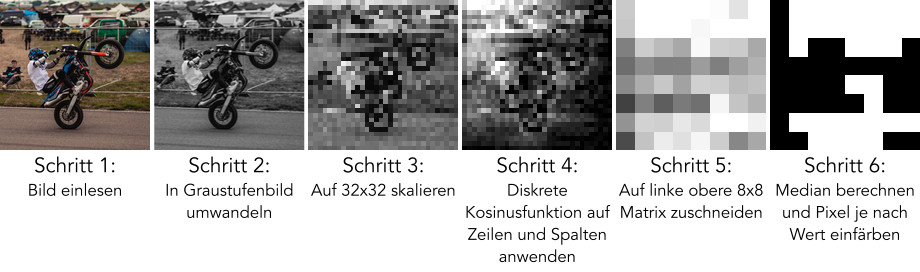
\includegraphics[width=\textwidth]{phash-process}
    \caption{PHASH: Schrittweise Berechnung des Hashes}
    \label{fig:phash-process}
    \bildquelle{Eigene Darstellung; Zugehöriger Programmcode im \hyperlink{page.14}{Anhang}}
\end{figure}

\noindent{\textbf{Vorteile}}
\begin{itemize}[topsep=0pt]
    \item Verhältnismäßig einfache Implementierung möglich
    \item Schnelle Suchperformance, wenn die Hashes der Referenzbilder bereits
    in einer dafür geeigneten Datenstruktur (z.B. \textit{k-d-Bäume}\footnote{https://www.cs.cmu.edu/~ckingsf/bioinfo-lectures/kdtrees.pdf [09.12.2022]},
    \textit{VP-Bäume}\footnote{https://fribbels.github.io/vptree/writeup [09.12.2022]}
    oder \textit{Kugelbäume}\footnote{https://towardsdatascience.com/tree-algorithms-explained-ball-tree-algorithm-vs-kd-tree-vs-brute-force-9746debcd940 [09.12.2022]})
    vorliegen \parencite{hashing-lvngd}
    \item Robust gegen Wasserzeichen, Farbfilter, leichte Helligkeits- und
    Kontraständerungen, Gammakorrekturen, Skalierungen sowie Komprimierungen
    (siehe Abbildung \ref{fig:phash})
    \parencite{hashing-phash}
\end{itemize}

\noindent{\textbf{Nachteile}}
\begin{itemize}[topsep=0pt]
    \item Nicht robust gegen Spiegelungen, Rotierungen und Verzerrungen (siehe
    Abbildung \ref{fig:phash})
    \item Nicht robust gegen Zuschneidungen, neu eingefügte Elemente oder
    Änderungen des Blickwinkels
\end{itemize}

\begin{figure}[H]
    \centering
    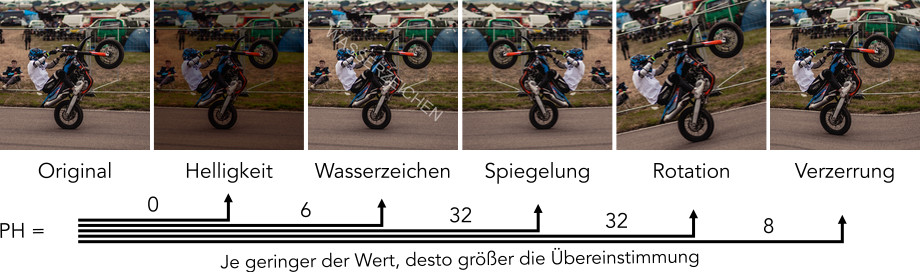
\includegraphics[width=\textwidth]{phash}
    \caption{PHASH: Anwendung an verschiedenen Testbildern}
    \label{fig:phash}
    \bildquelle{Eigene Darstellung}
\end{figure}

% Histogram Intersection
\newpage
\subsection{Histogram Intersection}
Ein robusteres, aber auch rechenaufwendigeres Verfahren ist der Histogram
Intersection Algorithmus von Swain und Ballard. Farbhistogramme sind stabil
gegenüber Spiegelungen, Verschiebungen und leichten Rotationen um die
Betrachtungsachse (siehe Abbildung \ref{fig:hintersection}). Außerdem ändern sie
sich bei Änderungen des Blickwinkels, des Maßstabs und bei Verdeckung von
Elementen nur langsam. Gegen Belichtungsänderungen können stark reduzierte
Farbhistogramme jedoch Probleme bereiten. \parencite{histogram-swain-ballard}

Im Standardfall wird das Histogram Intersection Verfahren auf Farbhistogramme
angewandt. Zuerst muss die Menge an zu diskretisierenden Farben im Histogramm
festgelegt werden - zum Beispiel 200. Das heißt, es gibt 200 mögliche
\glqq{}Farbeimer\grqq{} (Bins) in die jeder Pixel der Bilder einsortiert wird.
Nach dem Übereinanderlegen der durch das Referenz- und das Testbild berechneten
Histogramme wird schließlich deren Überschneidung berechnet. Je stärker sich
die Histogramme überschneiden, desto ähnlicher sind die Bilder
\parencite{histogram-image-similarity}. Zusätzlich wird wie beim Hashing ein
gewisser Schwellenwert vordefiniert. Der Vorgang kann beispielsweise auch auf
die einzelnen Farbkanäle aufgeteilt werden. Bei RGB würde das bedeuten, dass
jeweils der Rot-, Grün-, und der Blau-Kanal einzeln betrachtet wird.
\parencite{histogram-swain-ballard}

Eine weitere Untersuchung hat ergeben, dass sowohl die Wahl des Farbraums als
auch die Festlegung des Quantization Levels (Anzahl der Bins) eine große Rolle
bei der Erfolgsschance dieses Vorgehensmodells spielen. In dieser Studie
lieferte der CIELab-Farbraum im Allgemeinen die besten Ergebnisse.
\parencite{histogram-image-similarity}

Um die Genauigkeit des Algorithmus zusätzlich zu verbessern, können neben
Farbhistogrammen weitere Histogramme erstellt und verglichen werden. Ein
mögliches Beispiel wäre ein \glqq{}Texture Direction\grqq{} oder
\glqq{}Texture Scale\grqq{} Histogramm. In diesen Fällen wird nicht versucht
anhand der Farben eine Ähnlichkeit zu erkennen, sondern durch die Struktur des
Bildes. Hier werden beispielsweise aus dem Bild extrahierte Ecken oder Kanten in
ein Histogramm sortiert und schließlich auf Überschneidungen analysiert
\parencite{histogram-stackoverflow}. Jeder weitere zusätzliche
Berechnungsschritt wird dabei jedoch die Performance des Systems
beeinträchtigen.

\begin{figure}[H]
    \centering
    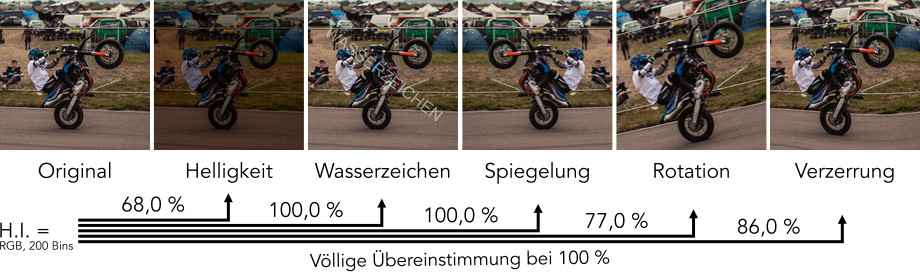
\includegraphics[width=\textwidth]{histogram-intersection}
    \caption{Histogram Intersection: Anwendung an verschiedenen Testbildern}
    \label{fig:hintersection}
    \bildquelle{Eigene Darstellung}
\end{figure}

% Scale-Invariant Feature Transform (SIFT)
\newpage
\subsection{Scale-Invariant Feature Transform (SIFT)}
David G. Lowe hat mit der Einführung des SIFT-Algorithmus einen für die
Bildverarbeitung wertvollen Beitrag geleistet. Der SIFT-Algoritmus findet lokale
Merkmale in Bildern. Diese Merkmale sind invariant gegenüber Bildskalierung und
-drehung und teilweise invariant gegenüber Änderungen der Beleuchtung sowie des
Betrachtungswinkels. Die Wahrscheinlichkeit einer Störung durch Verdeckung
einzelner Elemente oder auftretenden Bildrauschens wird, durch räumliche
Streuung und einem vielseitigen Frequenzbereich, erreicht. Im Folgenden wird die
grobe Vorgehensweise zur Findung der lokalen Merkmale erläutert.
\parencite{sift-distinctive-features}

\begin{enumerate}
    \item \textbf{Scale-space extrema detection}\newline
    Zu Beginn wird aus einem Bild durch repetetives Unschärfen (mittels
    \textit{Gaußschen Weichzeichner}\footnote{https://datacarpentry.org/image-processing/06-blurring/ [09.12.2022]})
    und Halbieren der Größe eine Serie an Bildern erzeugt (siehe Abbildung
    \ref{fig:sift1}). Auf die Bilder der Bilderserie folgt die Anwendung der
    \textit{Gaußschen Differenzfunktion}\footnote{https://www.sciencedirect.com/science/article/pii/B9780123694072500097 [09.12.2022]}
    (siehe Abbildung \ref{fig:sift2}). \parencite{sift-web-scale-space}

    \begin{figure}[H]
        \centering
        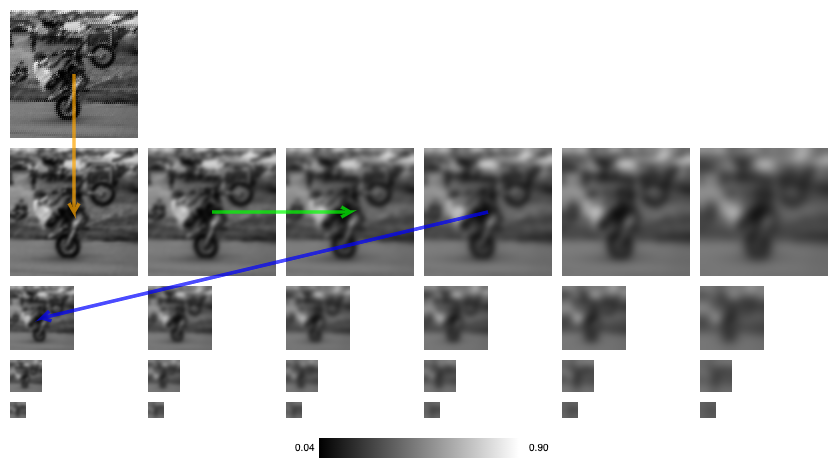
\includegraphics[width=13.3cm]{sift-1}
        \caption{SIFT: Erzeugung der Bilderserie}
        \label{fig:sift1}
        \bildquelle{Eigene Darstellung; http://weitz.de/sift/}
    \end{figure}

    \begin{figure}[H]
        \centering
        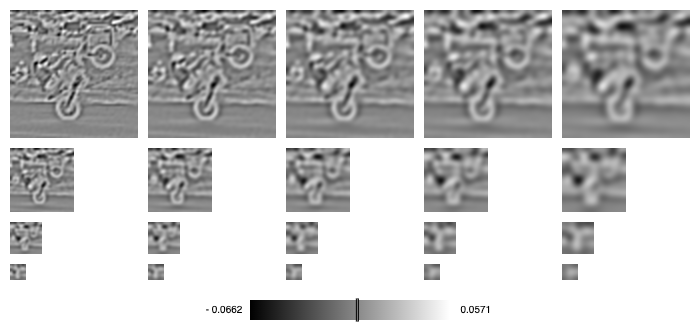
\includegraphics[width=13.3cm]{sift-2}
        \caption{SIFT: Anwendung Gaußscher Differenzfunktion}
        \label{fig:sift2}
        \bildquelle{Eigene Darstellung; http://weitz.de/sift/}
    \end{figure}

    \item \textbf{Keypoint localization}\newline
    Aus den vorher differenzierten Grafiken werden mit dem
    \textit{Marr-Hildreth-Operator}\footnote{https://theailearner.com/2019/05/25/laplacian-of-gaussian-log [09.12.2022]}
    interessante Schlüsselpunkte bzw. Merkmale herausgefiltert (siehe Abbildung
    \ref{fig:sift3}) \parencite{sift-web-keypoint}. Eine dem \textit{Harris-Corner-Detector}\footnote{https://docs.opencv.org/3.4/dc/d0d/tutorial\_py\_features\_harris.html [09.12.2022]}
    ähnliche Prozedur wird angewandt, um unwichtige Punkte herauszusieben
    (siehe Abbildung \ref{fig:sift5}) \parencite{sift-web-low-contrast}.

    \begin{figure}[H]
        \centering
        \begin{subfigure}{.5\textwidth}
          \centering
          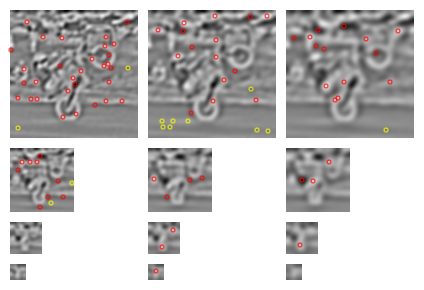
\includegraphics[width=.75\linewidth]{sift-3}
          \caption{Extrahierte Schlüsselpunkte}
          \label{fig:sift3}
        \end{subfigure}%
        \begin{subfigure}{.5\textwidth}
          \centering
          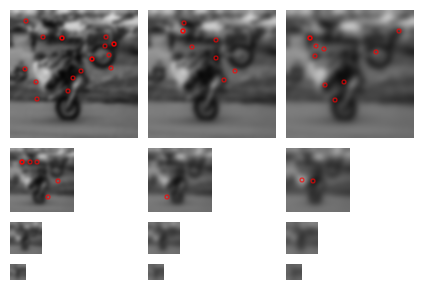
\includegraphics[width=.75\linewidth]{sift-5}
          \caption{Filterung unwichtiger Schlüsselpunkte}
          \label{fig:sift5}
        \end{subfigure}
        \caption{SIFT: Schlüsselpunkt-Lokalisierung}
        \label{fig:sift-keypoint}
        \bildquelle{Eigene Darstellung; http://weitz.de/sift/}
    \end{figure}

    \item \textbf{Orientation assignment}\newline
    Mithilfe eines Histogramms kann den Schlüsselpunkten nun eine Orientierung
    zugewiesen werden (siehe Abbildung \ref{fig:sift-orientation}). Dadurch
    werden die Punkte neben der Robustheit gegenüber Skalierung und Verschiebung
    auch gegen Rotation invariant (siehe Abbildung \ref{fig:sift}).
    \parencite{sift-web-orientation}

    \begin{figure}[H]
        \centering
        \begin{subfigure}{.5\textwidth}
          \centering
          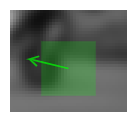
\includegraphics[width=.5\linewidth]{sift-6.png}
          \caption{Orientierung des Merkmals}
          \label{fig:sift6}
        \end{subfigure}%
        \begin{subfigure}{.5\textwidth}
          \centering
          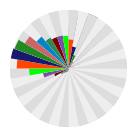
\includegraphics[width=.5\linewidth]{sift-6b.png}
          \caption{Zugehöriges Farbhistogramm (normalisiert)}
          \label{fig:sift6b}
        \end{subfigure}
        \caption{SIFT: Zuordnung der Orientierung}
        \label{fig:sift-orientation}
        \bildquelle{Eigene Darstellung; http://weitz.de/sift/}
    \end{figure}

    \item \textbf{Keypoint descriptor}\newline
    Zuletzt wird nach Anwendung weiterer mathematischer Verfahren eine Art
    Fingerabdruck des Merkmals berechnet (siehe Abbildung \ref{fig:sift7}).
    Dadurch wird die Stabilität gegenüber begrenzter lokaler Formverzerrungen
    und Beleuchtungsänderungen erreicht (siehe Abbildung \ref{fig:sift}).
    \parencite{sift-web-descriptor}

    \begin{figure}[H]
        \centering
        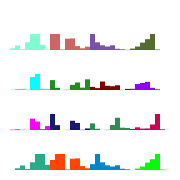
\includegraphics[width=5cm]{sift-7}
        \caption{SIFT: Pro Schlüsselpunkt erzeugte Deskriptoren (Fingerabdruck)}
        \label{fig:sift7}
        \bildquelle{Eigene Darstellung; http://weitz.de/sift/}
    \end{figure}
\end{enumerate}

Nach Anwendung dieses Algorithmus sollte man bei einem 500x500 Pixel großen Bild
mit rund 2000 robusten Merkmalen rechnen. Werden die gefundenen Merkmale in
einer Datenbank gespeichert, können sie in nahezu Echtzeit auf die
Schlüsselpunkte eines Testbilds verglichen werden.
\parencite{sift-distinctive-features}

Ein ähnlicher, jedoch bis 2033 patentierter\footnote{https://patents.google.com/patent/CN103640018A/en [09.12.2022]}, Algorithmus zur Erkennung von Bildmerkmalen ist der
\glqq{}Speeded up robust features (SURF)\grqq{} \parencite{sift-surf}. Ferner
gibt es viele ähnliche frei verfügbare Algorithmen der Gruppe
\glqq{}Bildmerkmalsfindung\grqq{}.

\begin{figure}[H]
    \centering
    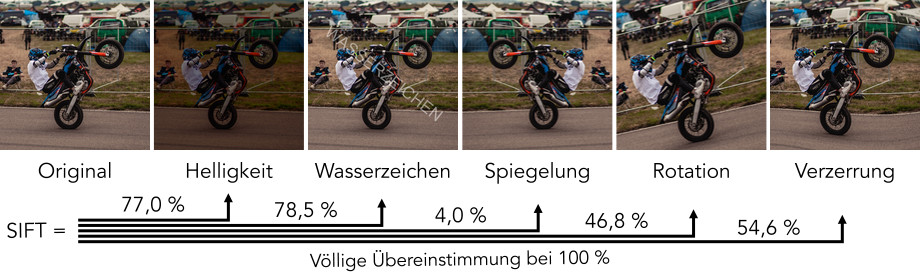
\includegraphics[width=\textwidth]{sift}
    \caption{SIFT: Anwendung an verschiedenen Testbildern}
    \label{fig:sift}
    \bildquelle{Eigene Darstellung}
\end{figure}


% Structural Similarity Index (SSIM)
\newpage
\subsection{Structural Similarity Index (SSIM)}
Anders als die meisten anderen Vorgehensmodelle versucht die menschliche
Wahrnehmung nicht Fehler zu Quantifizieren, sondern strukturelle Informationen
aus einer Szene wiederzuerkennen. Um dieses Verhalten nachzuahmen, haben
Forschende Mitglieder der IEEE den Structual Similarity Index entworfen.
\parencite{ssim-orig-paper}

\noindent{Der Index extrahiert, vergleicht und kombiniert folgende drei
Parameter:}
\begin{itemize}[topsep=0pt]
    \item Leuchtdichte
    \item Kontrast
    \item Struktur
\end{itemize}

Im ersten Schritt wird die Leuchtdichte durch Mittelwertbildung über alle
Pixelwerte gemessen. Anschließend wird der Kontrast durch Berechnung der
Standardabweichung aller Werte ermittelt. Vereinfacht dargestellt wird die
Struktur durch die Teilung des Eingangssignals durch seine Standardabweichung
geteilt, sodass eine genormte Standardabweichung entsteht.
\parencite{ssim-summary}

Sobald die drei Werte berechnet wurden, werden diese anhand, im Original-Paper,
veröffentlichten mathematischen Funktionen verglichen und schließlich
kombiniert. \parencite{ssim-summary}

Obendrein sei es nützlich den Index nicht global auf das Bild anzuwenden. Das
Paper gibt an den Algorithmus vorzugsweise auf verschiedene lokale Stellen
einzusetzen. Erstens seien für die Analyse interessante Objekte oft instationär
und zweitens können Bildverzerrungen auch räumlich variabel sein. Um die
Referenz zur Nachahmung der menschlichen Wahrnehmung zu ziehen, ist ebenfalls
festzustellen, dass Menschen ebenfalls nur lokale Bereiche einer Grafik in hoher
Auflösung wahrnehmen können. \parencite{ssim-summary}

Auch wenn der SSIM durch seine Einfachheit, gegenüber anderen Verfahren, eine
überragende Performance aufweist, ist der Algorithmus sehr anfällig für
Skalierungen, Verschiebungen und Rotierungen (siehe Abbildung \ref{fig:ssim}).
\parencite{ssim-quality-assessment}

\begin{figure}[H]
    \centering
    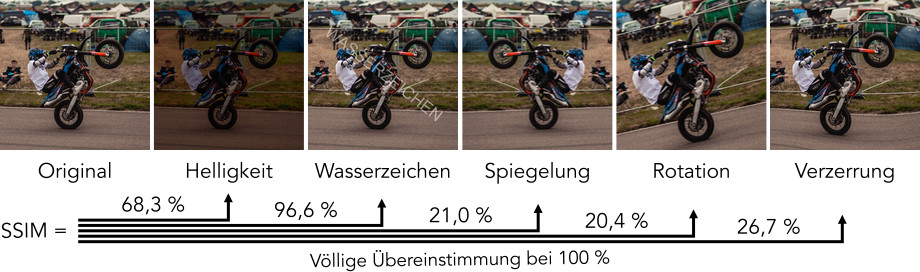
\includegraphics[width=\textwidth]{ssim}
    \caption{SSIM: Anwendung an verschiedenen Testbildern}
    \label{fig:ssim}
    \bildquelle{Eigene Darstellung}
\end{figure}


Aufbauend auf den SSIM-Algorithmus gibt es weitere optimierende Forschungen, wie
zum Beispiel der Complex Wavelet Structural Similarity Index. Der CW-SSIM
adressiert die vorher genannten Probleme und erzeugt durch Verwendung von
Wavelet-Transformationen eine Robustheit gegenüber kleinen Verschiebungen und
Rotierungen. \parencite{ssim-complex-wavelet}


% Fazit
\newpage
\section{Fazit und Ausblick}\label{fazit-u-ausblick}
Zusammenfassend bietet dieses Paper einen groben Überblick über den aktuellen
Forschungsstand bei der Ähnlichkeitsbestimmung von Bildern. Je nach Größe und
Art des Projekts eignen sich manche Algorithmen mehr und manche weniger. Eine 
allgemeingültige Lösung gibt es bisher nicht.

Der feingranulare inhaltsbasierte Vergleich zwischen Bildern wird auch
sicherlich in Zukunft noch ein wesentlicher Bestandteil der Forschung sein.
Neben den in der Einleitung \ref{einleitung} erläuterten Anwendungsfällen
spielen Image Matching Algorithmen insbesondere in der Medizin eine immer
größere Rolle. Beispielsweise sind computergestützte Diagnosen durch 
Bildvergleichsalgorithmen in der Lage Radiologen bei der Erkennung von
Krankheiten zu helfen \parencite{conclusion-medical}.

% Römische Nummerierung
\newpage
%\pagenumbering{Roman}
%\setcounter{page}{5}

% Literaturliste soll im Inhaltsverzeichnis auftauchen
\newpage
\phantomsection
\addcontentsline{toc}{section}{Quellenverzeichnis}
% Literaturverzeichnis anzeigen
\renewcommand\refname{Quellenverzeichnis}
\printbibliography


% Anhang
\newpage
\phantomsection
\appendix
\section*{Anhang}
\markboth{Anhang}{}
\addcontentsline{toc}{section}{Anhang}

\subsection*{Perceptual Hashing: Implementierung}
\noindent
Schrittweise Generierung eines Perceptual Hashes in Python unter der Verwendung
der OpenCV-Bibliothek.

\begin{lstlisting}[style=Python]
# Perceptual Hash Implementation by Andreas Huber
# Date: 2022-12-10
import numpy as np
import cv2

# Generates Perceptual Hash
def generatePerceptualHash(path, export=False):
    # Step 1: Read Image
    image = cv2.imread(path)
    if (export):
        cv2.imwrite('phash-results/phash-step-1.png', image)

    # Step 2: To grayscale	
    image = cv2.cvtColor(image, cv2.COLOR_BGR2GRAY)
    if (export):
        cv2.imwrite('phash-results/phash-step-2.png', image)

    # Step 3: To 32x32
    image = cv2.resize(image, (32, 32), interpolation = cv2.INTER_NEAREST)
    if (export):
        cv2.imwrite('phash-results/phash-step-3.png', image)

    # Step 4a: Discrete Cosinus Transform: Rows
    image = np.float32(image) / 255.0
    rows = cv2.dct(image, cv2.DCT_ROWS)
    
    # Step 4b: Discrete Cosinus Transform: Columns
    rows = cv2.rotate(rows, cv2.ROTATE_90_COUNTERCLOCKWISE)
    rows = cv2.flip(rows, 0)
    cols = cv2.dct(rows, cv2.DCT_ROWS)
    image = cv2.flip(cols, 0)
    image = cv2.rotate(image, cv2.ROTATE_90_CLOCKWISE)

    if (export):
        cv2.imwrite('phash-results/phash-step-4.png', image * 255)

    # Step 5: Crop to 8x8
    image = image[0:8, 0:8]

    if (export):
        cv2.imwrite('phash-results/phash-step-5.png', image * 255)

    # Step 6a: Calculate median
    imageValues = image.flatten()
    median = np.median(imageValues)

    # Step 6b: intensity < median ? black : white
    for i in range(8):
        for j in range(8):
            if (image[i][j] < median):
                image[i][j] = 0.0
            else:
                image[i][j] = 1.0

    if (export):
        cv2.imshow('resultHash', image)
        cv2.imwrite('phash-results/phash-step-6.png', image * 255)

    # Build string binary perceptual hash
    hash = image.flatten()
    hash = map(int, hash)

    if (export):
        cv2.waitKey(0)
        cv2.destroyAllWindows()

    return ''.join(map(str, hash))
\end{lstlisting}

\end{document}